\documentclass[12pt,reqno]{amsart}
\usepackage[top=2cm, left=2cm,right=2cm,bottom=2cm]{geometry}
\renewcommand{\baselinestretch}{1.2}
\usepackage{amsmath}
\usepackage{amssymb}
\usepackage{scalefnt}
\usepackage{tikz}
\usepackage{color,hyperref,enumerate,multicol}
\definecolor{darkblue}{rgb}{0.0,0.0,0.3}
\hypersetup{colorlinks,breaklinks,
            linkcolor=darkblue,urlcolor=darkblue,
            anchorcolor=darkblue,citecolor=darkblue}
            
\usepackage{algorithm}
\usepackage{algorithmic}
\pagestyle{empty}
\newcommand{\N}{\ensuremath{\mathbb{N}}}
\newcommand{\Z}{\ensuremath{\mathbb{Z}}}
\newcommand{\R}{\ensuremath{\mathbb{R}}}
\newcommand{\bL}{\ensuremath{\mathbf{L}}}
\newcommand{\bP}{\ensuremath{\mathbf{P}}}
\newcommand{\bQ}{\ensuremath{\mathbf{Q}}}
\newcommand{\bA}{\ensuremath{\mathbf{A}}}
\newcommand{\bB}{\ensuremath{\mathbf{B}}}
\newcommand{\bG}{\ensuremath{\mathbf{G}}}
\newcommand{\bH}{\ensuremath{\mathbf{H}}}
\newcommand{\invG}{\ensuremath{\operatorname{inv}^{\bG}}}
\newcommand{\invH}{\ensuremath{\operatorname{inv}^{\bH}}}
\newcommand{\meet}{\ensuremath{\wedge}}
\newcommand{\Meet}{\ensuremath{\bigwedge}}
\newcommand{\<}{\ensuremath{\langle}}
\renewcommand{\>}{\ensuremath{\rangle}}
\renewcommand{\phi}{\ensuremath{\varphi}}
\newcommand{\join}{\ensuremath{\vee}}
\renewcommand{\emptyset}{\ensuremath{\varnothing}}
\renewcommand{\subset}{\ensuremath{\subsetneq}}
\newcommand{\boldemph}{\emph}
\newcommand{\glb}{\operatorname{glb}}
\newcommand{\lub}{\operatorname{lub}}
\newcommand{\lcm}{\operatorname{lcm}}

\newcommand{\probskip}{\vskip1cm}

\begin{document}
\thispagestyle{empty}

\noindent \textbf{Math 301} \hskip3cm {\bf Homework 9 Solutions} \hfill {\bf Fall 2014}
\vskip1cm
\noindent {\bf Exercises:} 1, 2, 3 below and Judson: 9.22, 9.27, 9.31\\
{\bf Recommended:} 9.19, 9.21, 9.23, 9.41, 9.42, 9.45\\
{\bf Due date:} Friday, 10/31

\bigskip

\noindent The first few exercises require some definitions from lecture, 
repeated here for your convenience.

\vskip5mm

\noindent Let $\bA = \<A, F^{\bA}\>$ and $\bB = \<B, F^{\bB}\>$ be two algebras of the
same \emph{similarity type}.  That is, to each operation
symbol $f \in F$ there corresponds an operation $f^{\bA}$ defined on $\bA$ and an
operation $f^{\bB}$ defined on $\bB$.
Thus, the set of operations defined on $\bA$ is the set 
$F^{\bA} = \{f^{\bA} : f\in F\}$; similarly 
$F^{\bB} = \{f^{\bB} : f\in F\}$.

\vskip3mm

\noindent For example, any two groups $\bG$ and $\bH$ have the same similarity type. 
To emphasize this, we could denote the operations of these groups using
the precise (albeit somewhat awkward) notation of the previous paragraph, as follows:
\[
\bG  = \<G, \circ^{\bG}, \invG, e^{\bG}\> \quad \text{ and } \quad
\bH  = \<H, \circ^{\bH}, \invH, e^{\bH}\>.
\] 
Here $\circ^{\bG}$, $\invG$, and $e^{\bG}$ represent the \emph{interpretation
in} $\bG$ of the binary, unary (inverse), and  nullary (identity)
operations that a group must possess (similarly for $\bH$).  

\vskip5mm

\noindent An \emph{algebra homomorphism} (or simply \emph{homomorphism}), denoted by
$\varphi: \bA \rightarrow \bB$, is a function $\varphi$ with domain $A$ and
codomain $B$ that satisfies the following conditions: for each $f \in F$, if $f$
is an $n$-ary operation symbol, and if $a_1, \dots, a_n \in A$, then
\[
\varphi(f^{\bA}(a_1, \dots, a_n)) = f^{\bB}(\varphi(a_1), \dots, \varphi(a_n)).
\]

\vskip3mm

\noindent For example, a \emph{group homomorphism} $\varphi: \bG \rightarrow \bH$  is a function 
$\varphi$ with domain $G$ and codomain $H$ that satisfies, $\forall x, y \in G$,
\begin{enumerate}
\item  $\varphi(x\circ^{\bG} y) = \varphi(x) \circ^{\bH} \varphi(y)$,
\item  $\varphi(\invG(x)) = \invH(\varphi(x))$,
\item  $\varphi(e^{\bG}) = e^{\bH}$.
\end{enumerate}

\vskip5mm

\noindent The textbook defines a group \emph{isomorphism} to be a group homomorphism that is both
one-to-one and onto.  This definition is fine for algebraic structures (like
groups).  
It does not work, however, for relational structures, like posets. (See Exercise 3 below).
A definition that works for both algebraic and relational structures is the following:
A homomorphism $\varphi : \bA \rightarrow \bB$ is an \emph{isomorphism} if there
exists a homomorphism $\psi: \bB \rightarrow \bA$ that composes with
$\varphi$ to give the identity, that is,
$\varphi \circ \psi = \operatorname{id}_B$
and $\psi \circ \varphi= \operatorname{id}_A$. (Here, $\operatorname{id}_X$
denotes the identity function on the set $X$: $\operatorname{id}_X(x) = x$.)

\newpage

\noindent {\bf Exercises}

\begin{enumerate}[{\bf 1.}]
%% 1 %%%%%%%%%%%%%%%%%%%%%%%%%%%%%%%%%%%%%%%%%%%%%%%%
\item When discussing two groups, like $\bG$ and $\bH$ above,
  our textbook uses more convenient notation, such as 
  $(G, \cdot)$ and $(H, \circ)$ (or, even more simply, $G$ and $H$).  The book will then
  define a \emph{homomorphism} to be a function $\varphi: G\rightarrow H$ satisfying
  $\varphi(x\cdot y) = \varphi(x) \circ \varphi(y)$.
  Prove that this is equivalent to the definition given above by showing that 
  conditions (2) and (3) follow from condition (1).\\
  \ [Hint: Assuming (1), derive (3), then derive (2).]

\medskip
\noindent {\bf Solution:} 
We will be a little bit sloppy and rewrite the three conditions of our
definition as follows:
\begin{enumerate}[(1)]
\item
$\varphi(x\cdot y) = \varphi(x) \circ \varphi(y)$,
\item 
 $\varphi(x^{-1}) = [\varphi(x)]^{-1}$,
\item 
 $\varphi(e^{\bG}) = e^{\bH}$.
\end{enumerate}
since in each case the context makes clear whether we mean the operation in $\bG$ or
in $\bH$.
%% inverse we mean, and in (1)
%% it's clear that~$\cdot$ denotes the binary operation on $\bG$ and $\circ$ is
%% that on $\bH$.

\noindent
[(1) $\Rightarrow$ (3)]

%% \noindent
%% \underline{First proof:}
%% Assume (1) holds.
%%   Then, for any $x\in G$, 
%% \[
%% \varphi(x)  = \varphi(e^{\bG}\cdot x)  =
%% \varphi(e^{\bG})\circ \varphi(x) 
%% \]
%% and
%% \[\varphi(x)  = \varphi(x\cdot e^{\bG})  =
%% \varphi(x) \circ \varphi(e^{\bG}).
%% \]
%% Thus, for all elements $y\in H$ that happen to belong to the image of $G$ under
%% $\varphi$, we have 
%% \[
%% \label{eqn:1}
%% y\circ \varphi(e^{\bG}) = y = \varphi(e^{\bG}) \circ y.
%% \]
%% The image under $\varphi$ is nonempty, so there is at least one 
%% $y\in \varphi(G) \subseteq H$, and this element satisfies~(\ref{eqn:1}), so
%% \[
%% e^{\bH} \circ y = y = \varphi(e^{\bG}) \circ y.
%% \]
%% Multiplying both sides of this identity on the right by $y^{-1}$, we
%% have $e^{\bH}= \varphi(e^{\bG})$, so (3) holds.

\noindent
%% \underline{Alternative proof:} 
By~(1),
\[
\varphi(e^{\bG}) = \varphi(e^{\bG} \cdot e^{\bG}) = \varphi(e^{\bG}) \circ
\varphi(e^{\bG}).
\]
Multiplying on the right of both sides by $[\varphi(e^{\bG})]^{-1}$ yields
\[
e^\bH = \varphi(e^{\bG}) \circ [\varphi(e^{\bG})]^{-1} =
 \varphi(e^{\bG}) \circ \varphi(e^{\bG}) \circ [\varphi(e^{\bG})]^{-1}.
\]
Equivalently, $e^\bH = \varphi(e^{\bG})$.

\medskip

\noindent
[(1) and (3) $\Rightarrow$ (2)]

\noindent
Assuming (1) and (3) hold,
\[
e^{\bH} = \varphi(e^{\bG}) = 
\varphi(x\cdot x^{-1}) = 
\varphi(x)\circ \varphi(x^{-1}).
\]
Similarly, 
\[
e^{\bH} = \varphi(e^{\bG}) = 
\varphi(x^{-1}\cdot x) = 
\varphi(x^{-1}) \circ \varphi(x),
\]
which shows that, for each $x\in G$, the element $\varphi(x^{-1})$ is the
inverse of $\varphi(x)$.  That is, (2) holds.

\bigskip

%% 2 %%%%%%%%%%%%%%%%%%%%%%%%%%%%%%%%%%%%%%%%%%%%%%%%
\item
Define a lattice homomorphism.
Then consider a lattice $\bL = \<L, \meet, \join\>$ and a poset $\bP = \<P, \preccurlyeq\>$.
Is it possible to define a homomorphism $\varphi: \bL \rightarrow \bP$?  Explain.

\medskip
\noindent {\bf Solution:} 
A lattice  homomorphism is a function 
$\varphi: \bA \rightarrow  \bB$
from a lattice $\bA = \<A, \meet, \join\>$ to a
lattice $\bB = \<B, \meet, \join\>$,
that satisfies, for all $x, y \in A$, 
\[
\varphi(a\meet b)
=\varphi(a)\meet \varphi(b) 
\quad \text{
and }
\quad
\varphi(a\join b)
=\varphi(a) \join \varphi(b).
\]
(Again, the interpretation of the operations, $\meet$ and $\join$, depend on the
context.)

\medskip
It's not possible to define a homomorphism from the lattice $\bL$ to the poset
$\bP$ because these are not algebras of the same ``similarity type.''  To define
a homomorphism from an algebra $\bA$ to an algebra $\bB$, we first have to know
which operations of $\bA$ correspond to which operations of $\bB$.  
In the case where $\bA$ is a lattice and $\bB$ is a poset, we don't even have
the same \emph{number} of operations. In fact, the poset has no \emph{operations} at
all---it only has the \emph{relation} $\preccurlyeq$.

\emph{However}, as we learned in lecture, it may be the case that the poset
$\bP = \<P, \preccurlyeq\>$ has a special property---namely, that every pair 
$a, b \in P$ has a greatest lower bound and a least upper bound.  In that case,
we can define the binary operations $\meet$ and $\join$ on the poset as follows:
\[
x\meet y = \glb(x,y) \quad \text{ and } \quad x \join y = \lub(x,y),
\]
and then the poset becomes a lattice and we can talk about homomorphisms from
$\bL$ to $\bP$.
Conversely, every lattice (with operations $\meet$ and $\join$) is already a poset with
a partial order $\leq$ defined as follows:
\[
 x\leq y  \; \Longleftrightarrow \;  x\join y = x 
\quad \text{ and } \quad
x\leq y \; \Longleftrightarrow \;  x\meet y = x. 
\]
So, once we make this translation, it would then be possible to consider
\emph{poset homomorphisms} from $\bL$ to $\bP$.  (Poset
homomorphisms are defined and discussed in the next problem.)

\bigskip
%% 3 %%%%%%%%%%%%%%%%%%%%%%%%%%%%%%%%%%%%%%%%%%%%%%%%
\item
A \emph{poset homomorphism} is an order preserving map.  That is, if
$\bP = \<P, \leqslant\>$ and 
$\bQ = \<Q, \preccurlyeq\>$ are two partially 
ordered sets, then a homomorphism 
$\varphi: \bP \rightarrow \bQ$  is a function satisfying, for all $x, y\in P$, 
if $x \leqslant y$ then $\varphi(x)\preccurlyeq \varphi(y)$.
Consider the two definitions of \emph{isomorphism} given in the last paragraph
on Page 1 above.
Using the two posets shown below, explain why the first of these definitions is 
not appropriate for posets.

\vskip5mm

\begin{center}
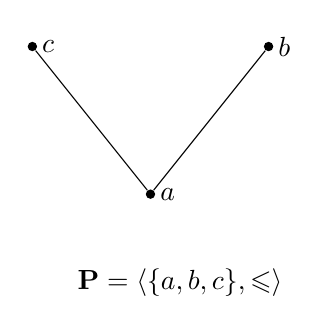
\begin{tikzpicture}[scale=0.75]
  \node (0) at (0,.5) [fill,circle,inner sep=1.2pt] {};
  \node (1) at (2,3) [fill,circle,inner sep=1.2pt] {};
  \node (2) at (-2,3) [fill,circle,inner sep=1.2pt] {};
  \draw (0) node [right] {$a$};
  \draw (1) node [right] {$b$};
  \draw (2) node [right] {$c$};
  \node (3) at (0.5,-1) {$\bP = \<\{a,b,c\},  \leqslant\>$};
  \draw (1) to (0) to (2);
\end{tikzpicture}
\hskip3cm
\begin{tikzpicture}[scale=0.75]
  \node (0) at (0,0) [fill,circle,inner sep=1.2pt] {};
  \node (1) at (0,2) [fill,circle,inner sep=1.2pt] {};
  \node (2) at (0,4) [fill,circle,inner sep=1.2pt] {};
  \draw (0) node [right] {$0$};
  \draw (1) node [right] {$1$};
  \draw (2) node [right] {$2$};
  \node (3) at (0.5,-1.5) {$\bQ = \<\{0,1,2\}, \preccurlyeq\>$};
  \draw (0) to (1) to (2);
\end{tikzpicture}
\end{center}


\noindent {\bf Solution:} The first definition says that an isomorphism is
simply a bijective homomorphism.  For the two posets shown above, we can
certainly find a bijective poset homomorphism, that is, an order preserving,
one-to-one, and onto function. For example, let 
$\phi(a) = 0$, 
$\phi(b) = 1$, and 
$\phi(c) = 2$. It's easy to see that this is an order preserving map:
$\phi(x) \preccurlyeq \phi(y)$ in $Q$ whenever 
$x\leq y$ in $P$.  However, $\phi$ fails to be a poset isomorphism since
the inverse map $\phi^{-1}$ is clearly not order preserving.  
For example, $1\preccurlyeq 2$ while $\phi^{-1}(1) = b  \nleq c = \phi^{-1}(2)$.

It should also be clear that any ``reasonable''
definition of isomorphism of posets should not characterize the two posets in the
diagrams above as isomorphic.  For one thing, the poset on the right is \emph{totally}
ordered while the one on the left is only partially ordered.
\vskip1cm

%% %% 7 %%%%%%%%%%%%%%%%%%%%%%%%%%%%%%%%%%%%%%%%%%%%%%%%
%% \item[{\bf 9.7.}] 
%% Show that any cyclic group of order $n$ is isomorphic to ${\mathbb Z}_n$. 

\newpage

\item[{\bf 9.22}]
Let $G$ be a group of order 20. If $G$ has subgroups $H$ and $K$ of
orders 4 and 5 respectively such that $hk = kh$ for all $h \in H$ and
$k \in K$, prove that $G$ is the internal direct product of $H$ and $K$. 

\medskip
\noindent {\bf Solution:}  
Assume $hk = kh$ for all $h\in H$ and $k\in K$.
Suppose $x \in H\cap K$. Then $x \in H$ implies $\<x\>$ is a subgroup of $H$ so,
by Lagrange's Theorem $|x|$ divides $|H| = 4$.
Similarly $x \in K$ implies $\<x\>$ is a subgroup of $K$ so,
by Lagrange's Theorem $|x|$ divides $|K| = 5$. Since $|x|$ divides both 4 and 5,
we must have $|x| = 1$, so $x = e$.  That is $H\cap K = \{e\}$.

To complete the proof, we must show $G = HK$.
Since $[G : K] = |G|/|K| = 20/5 = 4$, there are four cosets of
$K$ in $G$ and, since $H\cap K = \{e\}$, we can list these four cosets
using as representatives the four distinct elements of $H$. That is,
the cosets of $K$ in $G$ are $K, h_1K, h_2K, h_3K$.  Since any group is
the disjoint union of the cosets of any subgroup, we have
$G = K \cup h_1K \cup h_2K \cup h_3K = HK$.
 \qed

\vskip1cm

\item[{\bf 9.27}]
Let $G \cong H$. Show that if $G$ is cyclic, then so is $H$.

\medskip
\noindent {\bf Solution:} Suppose $G = \<a\> \cong H$ and suppose 
$\varphi: G \rightarrow H$ is an isomorphism.  Then 
$H = \<\varphi(a)\>$.  To see this, fix $h\in H$.  We will show 
$h = (\varphi(a))^k$ for some $k\in \N$. Indeed, let $b = \varphi^{-1}(h)$.
Since $b\in G = \<a\>$, we must have $b = a^k$ for some $k\in \N$.
Also, $\varphi(a^k) = (\varphi(a))^k$, since $\varphi$ is a homomorphism. 
Therefore, $(\varphi(a))^k = \varphi(a^k) = \varphi(b) = \varphi(\varphi^{-1}(h)) = h$.
\qed
\vskip1cm

\item[{\bf 9.31}]
Let $\phi : G_1 \rightarrow G_2$ and  $\psi : G_2 \rightarrow G_3$  be
isomorphisms. Show that  $\phi^{-1}$ and $\psi \circ \phi$ are both
isomorphisms. Using these results, show that the isomorphism of groups
determines an equivalence relation on the class of all groups.

\medskip
\noindent {\bf Solution:} First we show that $\phi^{-1}$ and $\psi\circ \phi$
are both homomorphisms.
Fix $u, v \in G_2$.  We must prove the homomorphism property:
\begin{equation}
  \label{eq:1}
\phi^{-1}(u \cdot v) = \phi^{-1}(u) \cdot \phi^{-1}(v).
\end{equation}
Since $\phi$ is onto, there exist $a, b\in G_1$ such that $\phi(a) = u$ and
$\phi(b) = v$.  Since $\phi$ is one-to-one, the inverse is well-defined and we
have $\phi^{-1}(u) = \phi^{-1}(\phi(a)) =a$ and 
$\phi^{-1}(v) = \phi^{-1}(\phi(b)) = b$.  Therefore,
\begin{align*}
\phi^{-1}(u  \cdot v) &= \phi^{-1}(\phi(a) \cdot  \phi(b))\\
&= \phi^{-1}(\phi(a \cdot  b)) \qquad \text{(since $\phi$ is a homomorphism)}\\
&= (\phi^{-1}\circ\phi)(a \cdot  b)\qquad \text{(by definition of function composition)}\\
&= a \cdot  b\\
&= \phi^{-1}(u) \cdot \phi^{-1}(v).
\end{align*}

Fix $x, y \in G_1$. We must prove the homomorphism property:
\begin{equation}
  \label{eq:2}
(\psi\circ \phi)(x\cdot y) =(\psi\circ \phi)(x)\cdot (\psi\circ \phi)(y).
\end{equation}
Indeed,
\begin{align*}
(\psi\circ \phi)(x\cdot y) &=\psi(\phi(x\cdot y)) \qquad \text{(by definition)}\\
&=\psi(\phi(x)\cdot \phi(y)) \qquad \text{(since $\phi$ is a homomorphism)}\\
&=\psi(\phi(x))\cdot \psi(\phi(y)) \qquad \text{(since $\psi$ is a homomorphism)}\\
&=(\psi\circ \phi)(x) \cdot (\psi\circ \phi)(y) \qquad \text{(by definition)}
\end{align*}
To finish the proof we must
show that $\phi^{-1}$ and $\psi\circ \phi$ 
are one-to-one and onto.\footnote{Since we are working with groups, the two
  definitions of isomorphism we gave at the bottom of page 1 are
  equivalent, so for groups we can take ``isomorphism'' to mean bijective
  homomorphism.} 
For the inverse function, these properties are obvious.  
As for $\psi \circ \phi$, suppose $x, y\in G_1$ and 
 $\psi(\phi (x)) =  (\psi(\phi(y))$. Then since $\psi$ is one-to-one we must
have $\phi(x)=\phi(y)$, and since $\phi$ is one-to-one, we have $x=y$, which
proves that $\psi\circ\phi$ is one-to-one.
To prove that $\psi\circ\phi$ is onto, let $z \in G_3$.  
Then since $\psi$ is onto, there exists $y\in G_2$ such that $\psi(y) = z$.
Since $\phi$ is onto, there exists $x\in G_1$ such that $\phi(x) = y$.
Therefore, $\psi\phi(x) = \psi(y) = z$, so 
$\psi\circ\phi$ is onto.

\medskip
Finally, we must show that $\cong$ determines an equivalence relation on the
class of all groups.
\begin{enumerate}
\item (reflexive) For every group $G$, we have $G \cong G$, since the identity
  map, $x \mapsto x$, is easily seen to be an isomorphism.
\item (symmetric) Assume $G \cong H$ and $\varphi: G \rightarrow H$ is an
  isomorphism. Then, by what we proved above, $\varphi^{-1}: H \rightarrow G$ is an isomorphism, so $H\cong G$.
\item (transitive) Assume $G \cong H$ and $H \cong K$.  We must show $G \cong K$. Let 
  $\varphi: G \rightarrow H$ and $\psi: H \rightarrow K$ be isomorphisms. Then, by what we proved above
 $\psi \circ \varphi: G \rightarrow K$ is an isomorphism so $G\cong K$.
\end{enumerate}
\end{enumerate}
\end{document}
